\section{Augmented Cube}
In this section, we calculated the full camera matrix in each frame and we used that for projecting a 3D cube into that frame. After that we tried to do the texture mapping on the faces of the cube we projected.

At first we started by checking pattern existence for each frame and if our implementation detect the chesspattern it will find the camera matrix of the current frame. For this, we used two different methods that we are going to explain and compare. In the first method we tried to find the camera matrix of the current view using the homography between the first and the second views. This method is the same one that we had implemented in the second assignment so we are not going into more details about it (for more detail read assignment 2).

In the second method instead of using two views, it calculates the camera matrix of the current view directly without using the first view. For this we used a function called GetObjectPos() in the SIGBTools that finds the object pose (rotation and translation) from the 3D-2D point correspondences.

The second method gives us a better result, probably because the first method computes the homography between two frames and because the frames can have relative distortion with each other and an absolute distortion it will give much worse result.

\begin{equation}
Method 1 = 
  	\begin{bmatrix}
			4.52461185e+02 &  4.68528179e+01 &  2.35842500e+02 &  3.39714824e+02 \\
			8.31252966e-01 &  5.27751638e+02 &  7.70575884e+01 &  2.88374192e+02 \\
			-1.69957230e-02 &  1.77008557e-01 &  6.93851813e-01 &  1.06122965e+00
		\end{bmatrix}
		\label{eq:cameramatrix1}
\end{equation}

\begin{equation}
Method 2 = 
		\begin{bmatrix}
			-5.61260110e+02 &  6.90221054e+01 &  3.29151908e+02 &  1.85913575e+04 \\
			-5.44911628e+00 & -5.17928968e+02 &  3.25490975e+02 &  1.90099438e+04 \\
			1.66644698e-02 &  1.78263033e-01 &  9.83841749e-01 &  4.90901087e+01
		\end{bmatrix}
		\label{eq:cameramatrix2}
\end{equation}

Now that we found the camera matrix with both methods for testing them we tried to project the chesspattern points in the world coordinate system to the current camera view. All points were projected to the right place in the image so we moved to the next step.
In this step we drew the world coordinate axes attached to the chesspattern plane and then we projected the cube into the current view again attached to the pattern plane. The cube projection only works fine with the second method and is totally shapeless in the first method. We could just have a perfect performance and accuracy in the second method.


 \begin{figure}[h!]
	\centering
	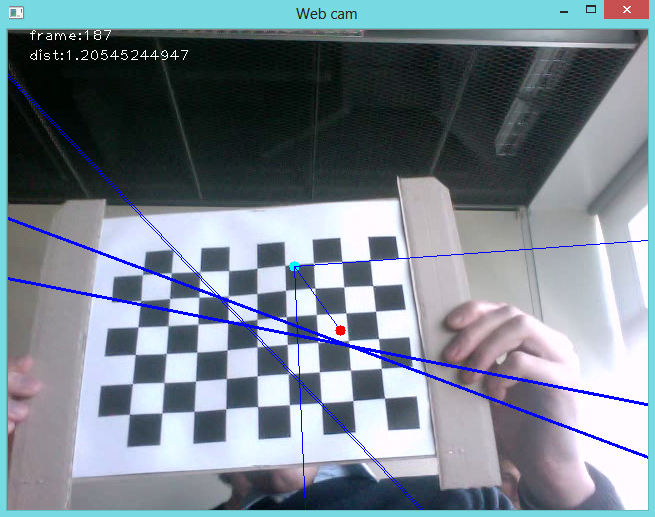
\includegraphics[width=11cm]{Handin3/images/method1.jpg}
	\caption{method1}
	\label{fig:method1}
\end{figure}
 \begin{figure}[h!]
	\centering
	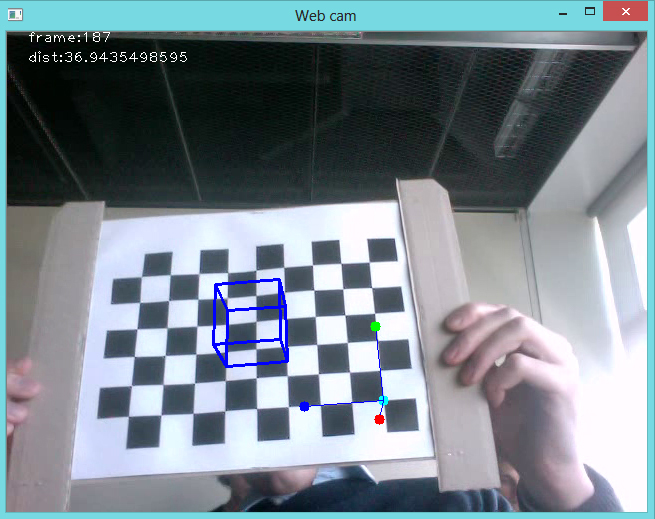
\includegraphics[width=11cm]{Handin3/images/method2.jpg}
	\caption{method2}
	\label{fig:method2}
\end{figure}

Last part of this section is texture mapping that we are going to do on the augmented cube. We used five images to mapping on the faces of the cube. For this we mapped each image by using the cube corners and calculating the homography matrix for each face of the cube.

 \begin{figure}[h!]
	\centering
	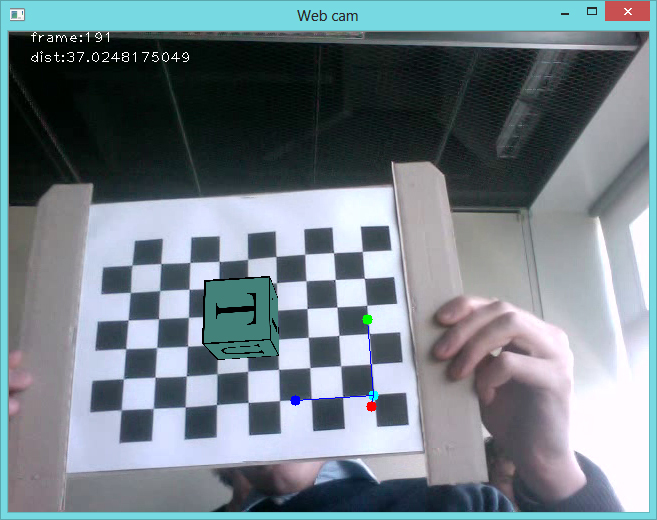
\includegraphics[width=11cm]{Handin3/images/texture.jpg}
	\caption{texture}
	\label{fig:texture}
\end{figure}
